\documentclass{report}


%%%%%%%%%%%%%%%%%%
%   Liste des packages utilisés  %
%%%%%%%%%%%%%%%%%%

\usepackage{amssymb}
\usepackage{array}
\usepackage{booktabs}
\usepackage{multirow}
\usepackage{float}
\usepackage{lmodern} %Pack de police
\usepackage{color}
\usepackage[dvipsnames]{xcolor}
\usepackage{graphicx}
\usepackage{svg}
\usepackage[utf8x]{inputenc}
\usepackage[T1]{fontenc}
%\usepackage{natbib}
\usepackage[square,sort,comma,numbers]{natbib}
\usepackage[francais,english]{babel}
\usepackage{caption}
\usepackage{listings}
\usepackage{booktabs}
\usepackage[top=2cm, bottom=2cm,left=2cm, right=2cm]{geometry}
\usepackage{blindtext}
\usepackage{setspace}
\usepackage{graphicx}
\usepackage{sidecap}
\usepackage{titlesec, blindtext, color} % titres spéciaux + couleur pour les chapter
\usepackage{fancyhdr}
\usepackage{seqsplit}
\usepackage[hyphens]{url}
\usepackage{lipsum}  
\usepackage{soul}

% on transforme les chapters en juste le numéro suivi du titre, avec un barre grisse
\definecolor{gray75}{gray}{0.75}
\newcommand{\hsp}{\hspace{20pt}}
\titleformat{\chapter}[hang]{\Huge\bfseries}{\thechapter\hsp\textcolor{gray75}{|}\hsp}{0pt}{\Huge\bfseries}


%\titleformat{\chapter}[display]
%	{\normalfont\huge\bfseries}{}{0pt}{\Huge}

\titlespacing*{\chapter}{0pt}{0pt}{15pt}
\titlespacing*{\subsection}{0pt}{2.0ex plus 1ex minus .2ex}{0.5ex plus .2ex}
\titlespacing*{\subsubsection}{0pt}{1.0ex plus 1ex minus .2ex}{0.5ex plus .2ex}


\makeatletter
\newcommand\footnoteref[1]{\protected@xdef\@thefnmark{\ref{#1}}\@footnotemark}
\makeatother


%Définition du style des bords de page
\pagestyle{fancy}
\renewcommand{\chaptermark}[1]{\markboth{\bsc{\thechapter{}- } #1}{}}
\lhead{}
\chead{}
\rhead{\leftmark}
\cfoot{}
\rfoot{Page \thepage}

\fancypagestyle{plain}{%
    \lhead{}
    \chead{}
    \rhead{}
    \renewcommand{\headrulewidth}{0pt}
    %\lfoot{Groupe n\up{o}2}
    \cfoot{}
    \rfoot{Page \thepage}
}

\begin{document}


%%%%%%%%%%%
%  Page de garde  %
%%%%%%%%%%%
\begin{titlepage}


		\begin{spacing}{1.5}
			\begin{minipage}{0.4\textwidth}
					
\includegraphics[width=3cm]{logo.png}\\
					Programmation interfaces embarquees\\
					Master Informatique – 1ere annee
			\end{minipage}
						\vspace*{\fill}

		\end{spacing}
	

	
	\begin{center}
		\begin{spacing}{2}
		    \hrule \vspace{1cm}
			\textbf{\Huge Android Project}\\[0.5cm]
			...
			\vspace{1cm}
			\hrule

			\vspace*{\fill}
		\end{spacing}

		\begin{spacing}{1.15}
			\vspace{12pt}
			Students: \\
			\textsc{Teyssier} Titouan\\
			\textsc{Pelloin} Valentin\\
			\vspace*{\fill}
		\end{spacing}

		\begin{spacing}{1.15}
			\today
			\vspace*{\fill}
		\end{spacing}
		
	\end{center}
\end{titlepage}



\tableofcontents


\chapter{Our application : Visual Life Configurator}
Our application is a cellular automaton simulation game. The player is free to create new automatons with the rules we want (for example Conway's game of life, Wireworld, ...).
For each automaton, the player configures how the automaton work, the types of cells, how neighbours are calculated, and the rules for a cell to be transformed into an other one.\\
Then, the player can create as many worlds he wants, edit them, and play with them.\\
Our application is called \texttt{VLC}, it stands for Visual Life Configurator.

\section{Persona}

\paragraph{Name}
John Doe
\paragraph{About}
John studies computer science. He is interested into algorithms and life simulation. John likes playing games on his phone while waiting for his bus before going to the University.
\paragraph{Goals}
\begin{itemize}
\item Learn new things
\item S
\end{itemize}

\section{User stories}
\begin{itemize}
	\item As a player, I want to entertain myself by playing a game ;
	\item As a user, I want to learn new ;
	\item As a player, I want to experiment new configurations of cellular automatons
\end{itemize}

\chapter{Functional study}

\section{Storyboards}

Below, the mock-ups of our application:
\vspace{12pt}

\begin{minipage}{.45\textwidth}
  \begin{minipage}{.45\linewidth}
    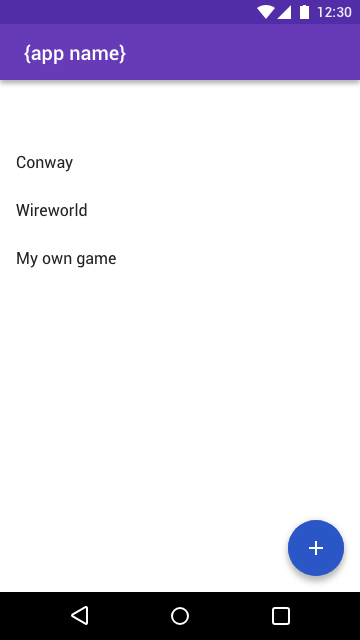
\includegraphics[width=\linewidth]{../mock-ups/Home.png}
  \end{minipage}\hfill
  \begin{minipage}{.45\linewidth}
    \captionof{figure}{The main activity of VLC. \\ The player can find all the automatons he created, and click on them to edit them or to play on a game.\\ The player can also click on the "plus" button to create and configure a new automaton.}
  \end{minipage}%
\end{minipage} \hfill
\begin{minipage}{.45\textwidth}
  \begin{minipage}{.45\linewidth}
    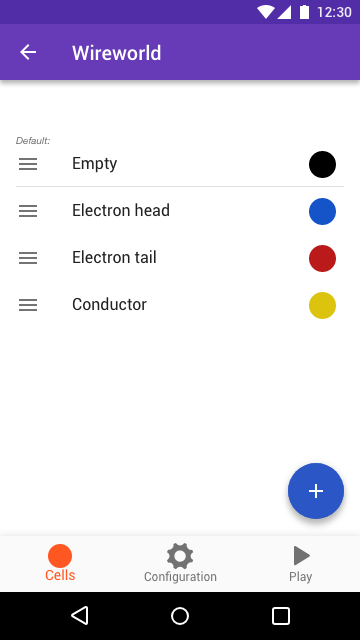
\includegraphics[width=\linewidth]{../mock-ups/Cells.png}
  \end{minipage}\hfill
  \begin{minipage}{.45\linewidth}
    \captionof{figure}{Inside a automaton, cells tab. \\ The player can create and remove cells types for this automaton. He can reorganize the order of the cells. The first cell type is the default one, the type of the cell that will fill the grid when creating a blank world.}
  \end{minipage}%
\end{minipage} \hfill


\begin{minipage}{.45\textwidth}
  \begin{minipage}{.45\linewidth}
    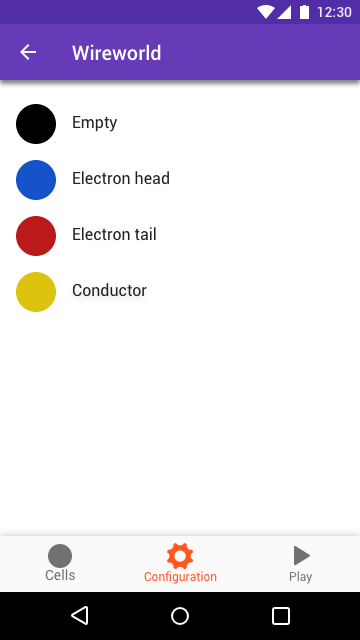
\includegraphics[width=\linewidth]{../mock-ups/Configuration.png}
  \end{minipage}\hfill
  \begin{minipage}{.45\linewidth}
    \captionof{figure}{Inside a automaton, configuration tab. \\ In this tab, the player can access the configuration for each cell.}
  \end{minipage}%
\end{minipage} \hfill
\begin{minipage}{.45\textwidth}
  \begin{minipage}{.45\linewidth}
    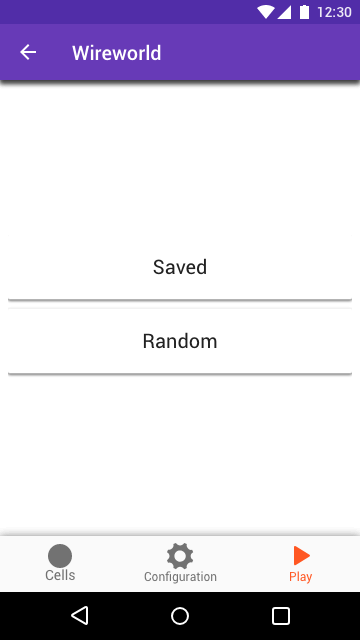
\includegraphics[width=\linewidth]{../mock-ups/Play.png}
  \end{minipage}\hfill
  \begin{minipage}{.45\linewidth}
    \captionof{figure}{Inside a automaton, play tab. \\ In this tab, the user can access to it's saved games. He can also choose to play on a random world.}
  \end{minipage}%
\end{minipage} \hfill


\begin{minipage}{.45\textwidth}
  \begin{minipage}{.45\linewidth}
    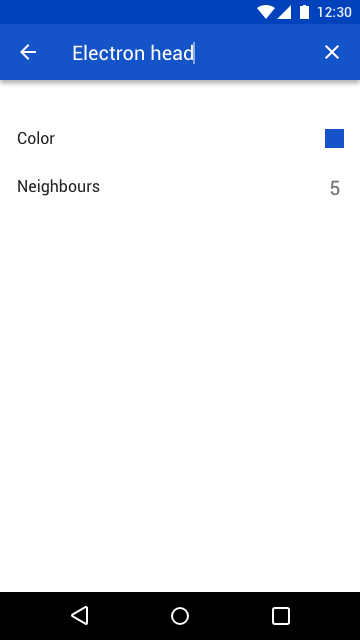
\includegraphics[width=\linewidth]{../mock-ups/Electron_head.png}
  \end{minipage}\hfill
  \begin{minipage}{.45\linewidth}
    \captionof{figure}{Cell parameter activity. \\ For this specific cell type, the user can edit its name, its color. He can also access to the neighbours choosing screen.}
  \end{minipage}%
\end{minipage} \hfill
\begin{minipage}{.45\textwidth}
  \begin{minipage}{.45\linewidth}
    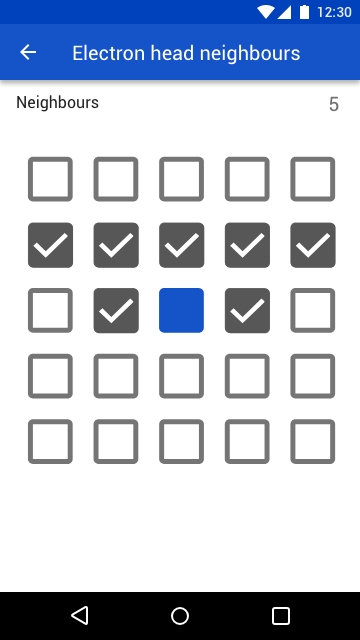
\includegraphics[width=\linewidth]{../mock-ups/Electron_head_neighbours.png}
  \end{minipage}\hfill
  \begin{minipage}{.45\linewidth}
    \captionof{figure}{Cell neighbours choosing. \\ On this activity, the player can choose which cells are being counted by the automaton as neighbours for this specific cell type.}
  \end{minipage}%
\end{minipage} \hfill


\begin{minipage}{.45\textwidth}
  \begin{minipage}{.45\linewidth}
    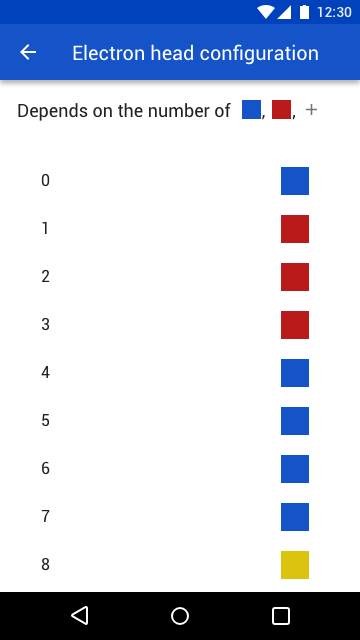
\includegraphics[width=\linewidth]{../mock-ups/Electron_head_configuration.png}
  \end{minipage}\hfill
  \begin{minipage}{.45\linewidth}
    \captionof{figure}{Cell type rule edition. \\ For this cell type (blue one), the player configured the rules of transformation. For example, if there are 8 neighbours around a blue cell, it will be transformed to a yellow cell in the next generation.}
  \end{minipage}%
\end{minipage} \hfill
\begin{minipage}{.45\textwidth}
  \begin{minipage}{.45\linewidth}
    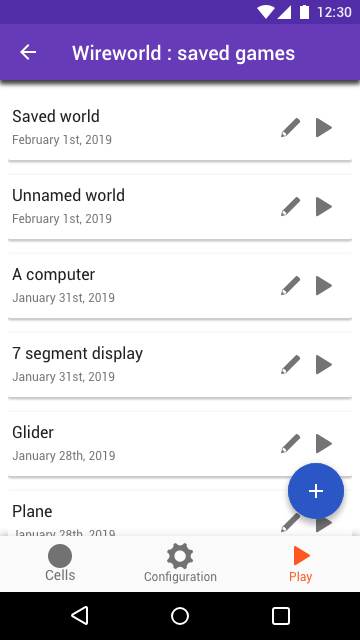
\includegraphics[width=\linewidth]{../mock-ups/Saved.png}
  \end{minipage}\hfill
  \begin{minipage}{.45\linewidth}
    \captionof{figure}{List of saved games. \\ The player can list worlds that are existing for a automaton. For each world, he can edit it, or play on it. By clicking on the "plus" button, e can also create a new blank world.}
  \end{minipage}%
\end{minipage} \hfill


\begin{minipage}{.45\textwidth}
  \begin{minipage}{.45\linewidth}
    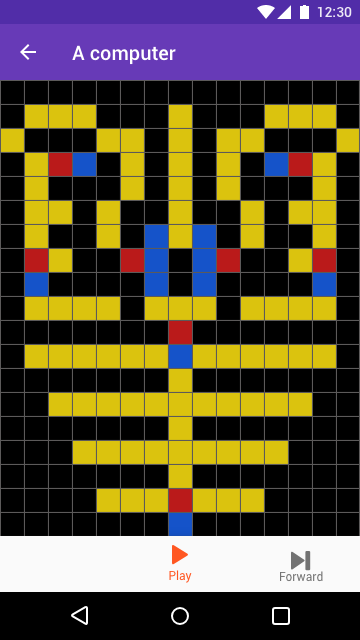
\includegraphics[width=\linewidth]{../mock-ups/Play_game_paused.png}
  \end{minipage}\hfill
  \begin{minipage}{.45\linewidth}
    \captionof{figure}{Playing game activity : paused. \\ By clicking on "Forward", the player can generate the next step.}
  \end{minipage}%
\end{minipage} \hfill
\begin{minipage}{.45\textwidth}
  \begin{minipage}{.45\linewidth}
    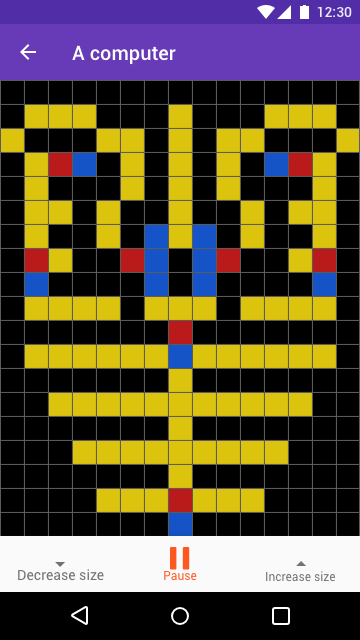
\includegraphics[width=\linewidth]{../mock-ups/Play_game_playing.png}
  \end{minipage}\hfill
  \begin{minipage}{.45\linewidth}
    \captionof{figure}{Playing game activity : playing. \\ The player can zoom in or zoom out.}
  \end{minipage}%
\end{minipage} \hfill


\begin{minipage}{.45\textwidth}
  \begin{minipage}{.45\linewidth}
    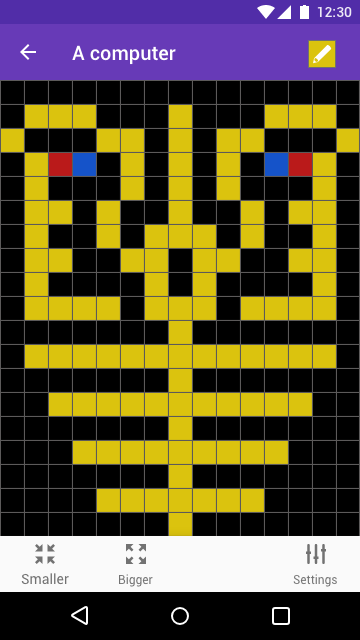
\includegraphics[width=\linewidth]{../mock-ups/Edit_game.png}
  \end{minipage}\hfill
  \begin{minipage}{.45\linewidth}
    \captionof{figure}{Editing a game. \\ The player can drag on cells to color them.}
  \end{minipage}%
\end{minipage} \hfill
\begin{minipage}{.45\textwidth}
  \begin{minipage}{.45\linewidth}
    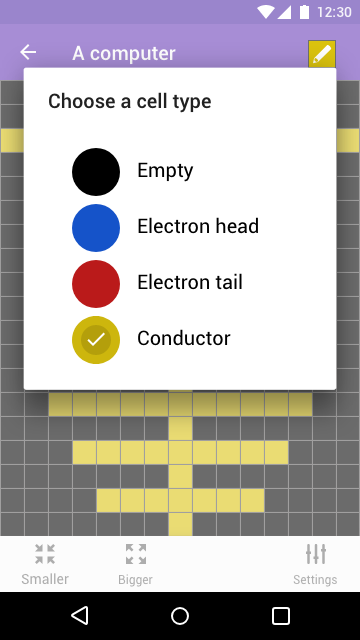
\includegraphics[width=\linewidth]{../mock-ups/Edit_game_popup.png}
  \end{minipage}\hfill
  \begin{minipage}{.45\linewidth}
    \captionof{figure}{Editing a game. \\ The player clicked on the pen in toolbar. He can change the color of cells he will be placing.}
  \end{minipage}%
\end{minipage} \hfill

\vspace{12pt}
It is possible to view a demonstration of these mock-ups by clicking on this

\section{Architecture}
d

\section{Github link}
Our project is accessible at \url{https://github.com/valentinp72/VisualLifeConfigurator}.

\end{document}